\documentclass{scrartcl}

\usepackage[ngerman]{babel}

\usepackage[utf8]{inputenc}
\usepackage{hyperref,xcolor,microtype,ifthen}
\usepackage{csquotes}

\usepackage{graphicx}
\usepackage{svg}

\usepackage{helvet}
\renewcommand{\familydefault}{\sfdefault}
\fontfamily{phv}\selectfont

\linespread{1.25}

\title{Mobile Application Lab}
\subtitle{Dokumentation der Quartett App}
\date{19.04.2017}
\author{Alexander Rasputin, Maximilian Karthan, Jona Ruof}

\begin{document}

\maketitle
\newpage
\tableofcontents

\section{Einleitung}
\subsection{Motivation}

Um die Besonderheiten bei der Entwicklung einer Applikation für eine mobile
Plattform kennenzulernen, sollte im Rahmen des Mobile Application Labs ein
Quartett Spiel für das Android System entwickelt werden. Da ein Spiel viele
verschiedene Aspekte einer Plattform benötigt und keine triviale Applikation
darstellt, erweist sich diese Problemstellung als geeignet für den Einstieg in
die Android Programmierung.

\ \newline
Außerdem konnten nur wenige Quartett-Apps gefunden werden, die nach gängigen
Kriteren als spielbar empfunden werden. So sind die meisten dieser Apps weder
optisch ansprechend noch performant oder intuitiv bedienbar. Kreative oder
innovative Ideen sind nur bei sehr wenigen Apps vorhanden. Auch die
Erweiterbarkeit und der generelle Umfang, also die Anzahl an spielbaren Karten,
ist meist sehr beschränkt. Zudem werden oft unnötigerweise für unterschiedliche
Thematiken der Quartett Karten zahlreiche Apps produziert die sich lediglich
in den verwendeten Graphiken unterscheiden. All diese Probleme motivierten somit
die Entwicklung einer echten Alternative für Quartett-Apps.

\subsection{Ziel}

Das hiermit erklärte Ziel dieses Projekts ist die Entwicklung einer Quarett-App,
welche die meisten der oben aufgelisteten Probleme der momementan verfügbaren
Apps löst oder diese zumindest entscheidend verbessert. Außerdem sollen
effektive Techniken für die Programmierung von Android Apps erabeitet werden.
Auch das Android API sollte nach Beendigung des Projekts im wesentlichen bekannt
sein. Besonderheiten im Umgang mit den begrenzten Ressourcen von mobilen
Plattformen sollten ebenfalls erlernt werden.

\ \newline
Die App selbst sollte dabei einen klassischen Einzelspieler Modus gegen einen
Computergegner und mindestens ein innovatives Feature aufweisen, um sich von der
Konkurrenz abzusetzen.

\subsection{Aufbau}

In der nun folgenden Dokumentation werden zuerst die Grundlagen des
Quartettspiels, der Android Plattform und die verwendeten Frameworks und
Libraries erklärt. Danach folgt eine Anforderungsanalyse, welche sowohl
funktionale als auch nicht funktionale Anforderungen umfasst. Im nächsten
Abschnitt werden einige wichtige Details der Implementierung sowie die
übergreifende Architektur und diverse Besonderheiten der App beschreiben.
Zuletzt werden die gestellten Anforderungen mit der tatsächlichen
Implementierung der App verglichen und es wird festgestellt welche Anforderungen
bis zu welchem Grad erfüllt wurden.

\section{Grundlagen}
\subsection{Quartettspiel}

Das klassische Quartettspiel ist bei Kindern ein beliebtes Kartenspiel. Das
Spielziel besteht darin möglichst viele Quartette, von vier zusammengehörigen
Karten zu sammeln. In unserer App spielen wir eine Abwandlung des klassischen
Quartetts, das sich Supertrumpf nennt bzw. im Umgangssprachlichen als
Autoquartett  bezeichnet wird. Im folgenden werden die Spielregeln und der
Spielverlauf eines Quartettspiels erklärt.

\subsubsection{Quartettkarte}

\begin{figure}[!ht]
\begin{center}
    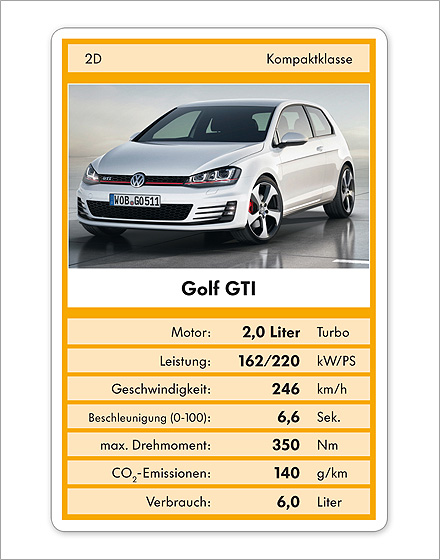
\includegraphics[scale=0.6]{img/quartett_card.jpg}
    \caption{Golf GTI Quartettkarte aus einem Autoquartett}
\end{center}
\end{figure}

In der oberen Abbildung wird eine Quartettkarte dargestellt. Deren Bild zeigt
einen Gegenstand, das zum Gengere des Quartettdecks passt, in unserem Fall ein
Auto, das zu einem Autoquartett gehört. In der Mitte befindet sich der Name des
Gegenstandes, hierbei handelt es sich um einen Golf GTI. Der untere Teil besteht
aus Attributen mit ihren Attributwerten, die im Spielverlauf verglichen werden.

\subsubsection{Spielverlauf}

Am Spiel nehmen zwei Personen teil, der Benutzer der App ein Computergegener
oder über den Multiplayer eine weitere Person. Der Benutzer entscheidet sich für
ein Quartett. Die Karten werden gemischt und gleichmäßig unter den beiden
Spielern verteilt. Beide Spieler haben nun einen umgedrehten Stapel an Karten.
Die oberste Karte ist aufgedeckt, diese Karte ist nur für die jeweilige Person
sichtbar. Der Benutzer wählt ein Attribut der Karte aus, das er mit der anderen
Person vergleichen möchte. Nun werden die Werte der beiden Attribute verglichen.
Gewinner der Runde ist die Person, die den besseren Attributswert hat. Dieser
gewinnt die Karte. Klassisch wird gespielt bis einer der beiden Personen keine
Karten mehr hat.

\begin{figure}[!ht]
\begin{center}
    \includegraphics[scale=0.6]{img/map_quartett.png}
    \caption{Darstellung eines Quartettspielverlaufes}
\end{center}
\end{figure}

In unserem Fall haben wir uns gegen den klassischen Spielmodus entschieden, da
dieser im Kontext einer Mobilen Anwendung ungeeignet ist. Gründe dafür sind,
z.B. die relative Länge eines Spieles.
\newline
Daher haben wir uns für 4 unterschiedlichen Spielmodi entschieden die im
Nachfolgenden erklärt werden.

\subsubsection{Spielmodi}

\textbf{Rundenbasiert:}
Gewonnen hat derjenige, mit den meisten gewonnenen Runden. Zu berücksichtigen
ist das Rundenlimit, das vor Spielbeginn gesetzt wird.

\ \newline
\textbf{Punktebasiert}:
Vor dem Spiel wird eine Punktegrenze bestimmt. Gewinner ist derjenige, der diese
Punktegrenze zuerst erreicht hat.

\ \newline
\textbf{Zeitbasiert:}
Es wird ein Zeitlimit vor dem Spiel gesetzt. Gewonnen hat die Person, die
am meisten Punkte erreicht hat, bevor dass Zeitlimit abgelaufen ist.

\subsection{Mobile Plattform}
Der Kerngedanke dieses Projekts war das Kennenlernen einer Mobilen Plattform und
ihrer Besonderheiten im Zusammenhang mit der Anwendungsentwicklung für diese
Plattform. Wir haben uns für Android als Zielplattform entschieden.

\ \newline
Die wichtigsten Eigenarten von Android, im Vergleich zu der Entwicklung von
Software auf Computern, sind das sogenannte Sandbox-Prinzip des Betriebssystems,
die viel größere Abhängigkeit von Multithreading für ein performantes System und
die sogenannten Activities und deren Lifecycle.

\ \newline
Kommen wir zunächst zu Androids Sandbox-Prinzip. Android führt Anwendungen in
einer Sandbox aus, einer eingeschränkten Laufzeitumgebung, in der bestimmte
Funktionen verboten sind. Dazu gehört beispielsweise der direkte Zugriff auf
Daten einer anderen Anwendung. Dies führt dazu, dass Anwendungen Berechtigungen
einholen müssen um beispielsweise eine Internetverbindung aufzubauen oder eine
SMS zu verschicken. Diese Berechtigungen werden im Android-Manifest gepflegt,
sodass diese dem System zum Installationszeitpunkt bereits bekannt sind. Während
der Entwicklung ist man immer wieder auf das Problem gestoßen, dass man
vergessen hat die entsprechenden Berechtigungen zu setzen.

\ \newline
Besonders wichtig war während der Entwicklung, niemals zu viel Arbeit auf dem
Main-Thread zu erledigen. Der Main-Thread, in der Android Welt auch UI-Thread
genannt, ist der Thread der sich vor allem um das User Interface kümmert, in Form
von Eventhandling und Interaktionen mit Views im User Interface. Alle
Komponenten, die gestartet werden, laufen standardmäßig auf diesem Thread. Wird
nun vom Programmierer nicht darauf geachtet diesen Thread nicht zu überlasten,
kann er nicht mehr genug Leistung erbringen um die Views auf dem User Interface
flüssig zu animieren oder um sofort auf Benutzereingaben zu reagieren. Diese
Verzögerungen fallen dem Benutzer bei Geräten mit Touchscreens als Eingabemedium
besonders auf. Durch die spezielle Art der Eingabe ist es überaus wichtig dafür
Sorge zu tragen, dass das User Interface stets auf Eingaben durch den Benutzer
reagiert.

\ \newline
Android wurde dafür konzipiert um auf Smartphones und Embedded Systemen zu
laufen. Da diese Geräte im Vergleich zu modernen PCs kleine Prozessoren und
wenig Hauptspeicher haben und meist auch noch mit einem Akku als Stromquelle
laufen, welcher bei intensivem Gebrauch schnell erschöpft ist mussten sich die
Android Entwickler etwas ausdenken, um dem Rechnung zu tragen. Ihre Lösung war,
dass Android in die Lebensdauer von Komponenten einer Anwendung und von
Prozessen eingreift. Im Falle knapper Ressourcen können einzelne Activities,
Services oder auch ganze Prozesse beendet werden. Diesem Umstand müssen wir als
Programmierer wiederum Rechnung tragen, da wir davon ausgehen müssen, dass
unsere Komponenten zur Laufzeit beendet werden. Um Datenverlust zu vermeiden
bietet uns Android jedoch den sogenannten Activity Lifecycle. Das Betriebssystem
\enquote{verspricht} uns sozusagen, dass gewisse Methoden einer Activity in
bestimmter Reihenfolge durchlaufen werden wenn diese beendet wird oder eben auch
wenn diese wieder neu gestartet wird.

\subsection{Libraries und Frameworks}
Um einige Funktionen der Applikation nicht selbst implementieren zu müssen
wurden folgende zusätzliche Programmbibliotheken und Frameworks verwendet:

\noindent
\ \newline
\textbf{Sugar ORM, http://satyan.github.io/sugar/} \newline
Eine sehr einfach zu konfigurierende ORM Bibliothek, welche allerdings nur
simple Relationen abbilden kann. Sugar ORM wurde verwendet um die interne SQLite
Datenbank des Android Systems direkt über Objekte anzusprechen. Somit mussten
keine SQL Befehle zur Steuerung der Datenbank verwendet werden.

\ \newline
\textbf{Volley, https://github.com/google/volley} \newline
Volley ist eine Netzwerkbibliothek welche die Kommunikation mit Webservices
erheblich erleichtert. Alle requests und responses werden asynchron behandelt
und als abstrakte Objekte repräsentiert. Diverse Datenformate (wie JSON) werden
direkt in einer Objektrepräsentation ausgegeben und sind somit im Programm ohne
weitere Umwandlung zugänglich. Auch das direkte Laden von Bildern in Widgets
(z.B. ImageView) und das dazugehörige Caching wird von Volley übernommen. Volley
wurde verwendet um die Kommunikation mit dem bereitgestellten Quartett Server zu
implementieren.

\ \newline
\textbf{FlippableStackView, https://github.com/blipinsk/FlippableStackView} \newline
Diese Bibliothek stellt ein Widget bereit, in welchem einzelne Views wie in
einem Kartendeck durchgeblättert werden können. FlippableStackView wurde
verwendet um die Detailansicht eines Decks in der Galerie zu erstellen.

\ \newline
\textbf{CircleProgress, https://github.com/lzyzsd/CircleProgress} \newline
CircleProgress stellt eine Reihe an kreisförmigen Fortschrittsanzeigen bereit.
Diese wurden verwendet um die Anzeige der Spielstatistiken zu realisieren.

\newpage
\ \newline
\textbf{Android Image Cropper, https://github.com/ArthurHub/Android-Image-Cropper} \newline
Android Image Cropper stellt eine Ansicht bereit in welcher zuvor aufgenommen
Bilder zugeschnitten und gedreht werden können. Diese Bibliothek wurde zur
Implementierung des Profilbilds in den Spieleinstellungen verwendet.

\ \newline
\textbf{CircleImageView, https://github.com/hdodenhof/CircleImageView} \newline
Diese Bibliothek beinhaltet ein modifiziertes ImageView Widget, welches statt
einem Rechteck einen Kreis als Grundfläche besitzt. Mit Hilfe von
CircleImageView wurde die Anzeige des Profilbilds in den Spieleinstellungen und
im Navigation Drawer realisiert.

\ \newline
\textbf{Google Play Services API, https://developers.google.com/games/services/} \newline
Diese Framework ermöglich den Zugriff auf die Google Play Services und somit
eine einfache Online-Anbindung für Spiele. Neben einem Programmiermodell für
Multiplayerspiele stellt das Framework auch Ranglisten, ein Freundesystem und
Einladungen für Spiele bereit. Die Google Play Services wurden für den
Multiplayer der App verwendet.


\section{Anforderungsanalyse}
\subsection{Funktionale Anforderungen}

Im folgenden werden alle funktionalen und nicht funktionalen Anforderungen
aufgelistet, die vor oder während der Entwicklung der Applikation gestellt
wurden.

\ \newline
\textbf{FA1 Hauptmenü} \newline
Der Benutzer kann von einem Hauptmenü, welches nach Start der App angezeigt
wird, schnell auf die wichtigsten Funktionen der App zugreifen.

\ \newline
\textbf{FA2 Spielmodi} \newline
Der Benutzer kann vor jedem Spiel aus 4 verschiedenen Spielmodi wählen:
Zeitspiel (Spielende nach Ablauf eines Zeitlimits), Punktspiel (Spielende bei
bestimmter Punktezahl), Rundenspiel (Spielende nach bestimmter Anzahl Runden),
Insane (Vergleiche umgekehrt, Spielende nach bestimmter Anzahl Runden).

\newpage
\ \newline
\textbf{FA3 Computergegner} \newline
Im Einzelspieler Modus kann der Benutzer gegen einen simulierten Gegner
antreten. Dieser sollte sich wie ein menschlicher Spieler verhalten und nicht
auf Informationen zurückgreifen können, die einem menschlichen Gegner
normalerweise nicht zur Verfügung stehen. So sollten z.B. die Werte der Karte
des Benutzers dem Computergegner nicht für die Planung des Spielzugs zur
Verfügung stehen. So soll ein \enquote{unfaires} Verhalten und damit ein
frustrierendes Spielerlebnis verhindert werden.

\ \newline
\textbf{FA4 Schwierigkeitsgrad} \newline
Vor jedem neuen Spiel kann der Benutzer einen von 3 verschiedene
Schwierigkeitsgraden (Leicht, Mittel, Schwer) wählen. Je nach gewähltem
Schwierigkeitsgrad handelt der Computergegner mehr oder weniger intelligent.

\ \newline
\textbf{FA5 Spiel fortsetzen} \newline
Der gesamte Spielfortschritt wird kontinuierlich in der Applikation persistent
gespeichert. So kann auch nach einem Neustart der App das Spiel ohne
Fortschrittsverlust fortgesetzt werden.

\ \newline
\textbf{FA6 Galerie} \newline
Alle im Spiel vorhandenen Quartettdecks lassen sich in einer speziellen Ansicht,
der Galerie, betrachten. Dabei können alle im Deck enthaltenen Karten einzeln
in einer detaillierten Ansicht betrachtet werden.

\ \newline
\textbf{FA7 Deck Download} \newline
Die Applikation erlaubt das Herunterladen weiterer Kartendecks von einem
externen Server. Nach dem Herunterladen können diese Decks, genauso wie die
bereits in der App vorhandenen Decks, im Spiel verwendet werden. Die Decks werden
persistent gespeichert und sind somit nach erfolgreichem Download auch ohne
Internetverbindung dauerhaft verfügbar.

\ \newline
\textbf{FA8 Statistiken} \newline
Die App sammelt während der Laufzeit spielbezogene Daten, um Statistiken zu
ermöglichen. Diese Statistiken können vom Spieler in einer speziellen Ansicht
eingesehen werden. Mögliche Statistiken sind: kill / death ratio, höchste
Gewinnserie, höchste Verlustserie

\ \newline
\textbf{FA9 Rangliste} \newline
Es gibt eine Rangliste, in welcher der Benutzer die im Spiel erhaltenen Punkte
mit seinem Namen publizieren kann.

\ \newline
\textbf{FA10 Achievements} \newline
Die App beinhaltete ein Achievementsystem. Wenn gewissen Herausforderungen
erfüllt werden, können Achievements freigeschaltet werden und in einer
speziellen Ansicht angesehen werden.

\ \newline
\textbf{FA11 Quartetteditor} \newline
Es wird ein Quartetteditor bereitgestellt, der es dem Benutzer ermöglich
eigene Quartettdecks zu erstellen. Mit den erstellen Decks kann wie mit den
bereits im Spiel integrierten Decks gespielt werden.

\ \newline
\textbf{FA12 Levelsystem} \newline
Ein Levelsystem suggeriert permanenten Fortschritt. Nach jedem Spiel erhält der
Benutzer Erfahrungspunkte, welche das Level steigen lassen. Mit diesem System
soll eine Langzeitmotivation erreicht werden.

\ \newline
\textbf{FA13 Multiplayer} \newline
Es ist über ein Netzwerk möglich gegen andere Benutzer der App anzutreten.


\subsection{Nicht Funktionale Anforderungen}

\textbf{NFA1 Robustheit} \newline
Das Spiel soll eine gewisse Robustheit aufweisen, also auf fehlerhafte Eingaben
oder unvorhergesehene Ereignisse angemessen reagieren. Im Falle eine Absturzes
sollte die Applikation ohne Verlust des Spielfortschritts neu gestartet werden
können.

\ \newline
\textbf{NFA2 Erweiterbarkeit} \newline
Die Programmstruktur der Applikation sollte derart gestaltet sein, dass
spätere Erweiterungen möglichst einfach vorgenommen werden können.

\newpage
\ \newline
\textbf{NFA3 Responsiveness} \newline
Die Oberfläche sollte stets innerhalb einer sehr kurzen Zeit auf
Benutzereingaben reagieren. Bei längeren Wartezeiten, etwa während eines
Downloads, sollte der Benutzer permanent, durch den Einsatz von entsprechenden
GUI-Elementen, über den Fortschritt der Operation informiert werden.

\ \newline
\textbf{NFA4 Usability} \newline
Der Benutzer sollte die App, nach einer kurzen Einführung, durch eine intuitive
und benutzerfreundliche Oberfläche ohne weitere Anleitung bedienen können.

\section{Konzept und Entwurf}
\subsection{Mockups}
Vor dem eigentlichen Implementieren der App wurden Mockups erstellt. Diese
sollten einen ersten Eindruck vom User Interface geben und dienten als
Orientierung während der eigentlichen Implementierung.

\begin{figure}[!ht]
\begin{center}
	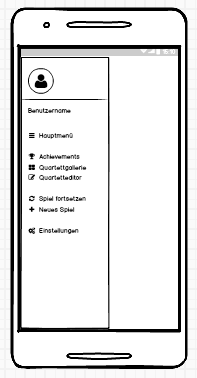
\includegraphics[scale=0.67]{img/mockup_drawer.png}
	\caption{Navigation Drawer}
	\label{drawer}
\end{center}
An jeder beliebigen Stelle der App hat man Zugriff auf den Navigation Drawer.
Dieser ist ein Menü, welches sich von der linken Seite durch eine Wischgeste
herausziehen lässt. Abbildung ~\ref{drawer} zeigt das Konzept dieses Menüs.
\end{figure}

\begin{figure}[!ht]
\begin{center}
	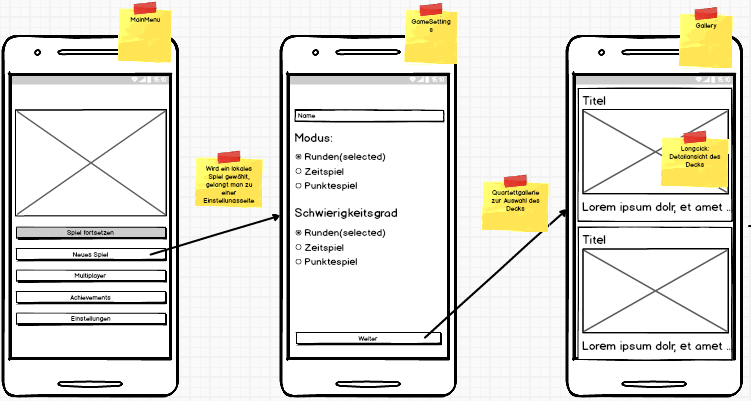
\includegraphics[scale=0.7]{img/mockup_game_process_1.png}
	\caption{Singleplayer Einstellungen}
	\label{singleplayer1}
\end{center}
Abbildung ~\ref{singleplayer1} skizziert den Prozess, welchen der Benutzer
vollführen muss, um vom Hauptmenü zum Einzelspieler Modus zu gelangen.
\end{figure}

\vspace{1cm}

\begin{figure}[!ht]
\begin{center}
	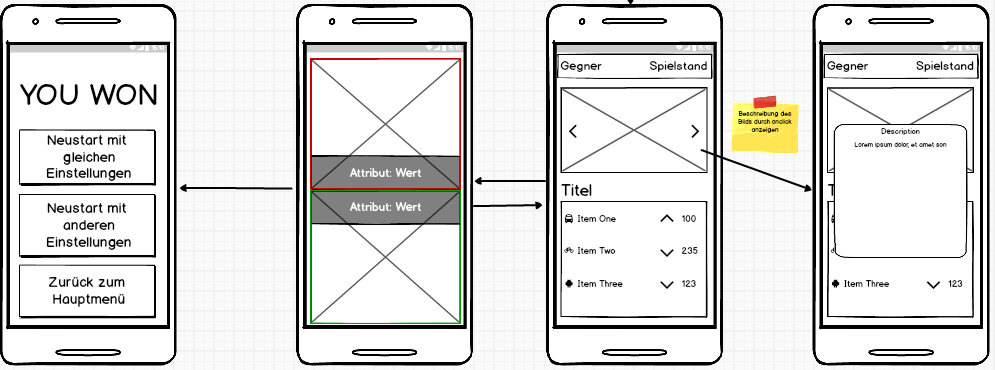
\includegraphics[scale=0.55]{img/mockup_game_process_2.png}
	\caption{Singleplayer}
	\label{singleplayer2}
\end{center}
Nach dem das Deck ausgewählt wurde befindet sich der Spieler im eigentlichen
Einzelspieler Modus. Abbildung ~\ref{singleplayer2} skizziert das
Spielgeschehen.
\end{figure}

\begin{figure}[!ht]
\begin{center}
	\centering
	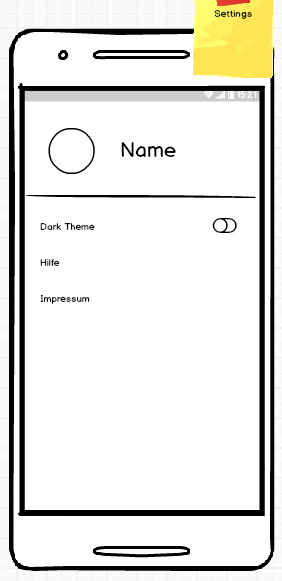
\includegraphics[scale=0.4]{img/mockup_settings.png}
	\caption{Settings Activity}
	\label{settings}
\end{center}
Einstellungen kann der Benutzer in der Settings Activity vornehmen. Allerdings
sind die Möglichkeiten in unserer App sehr beschränkt wie Abbildung
~\ref{settings} zeigt.
\end{figure}

\begin{figure}[!ht]
\begin{center}
	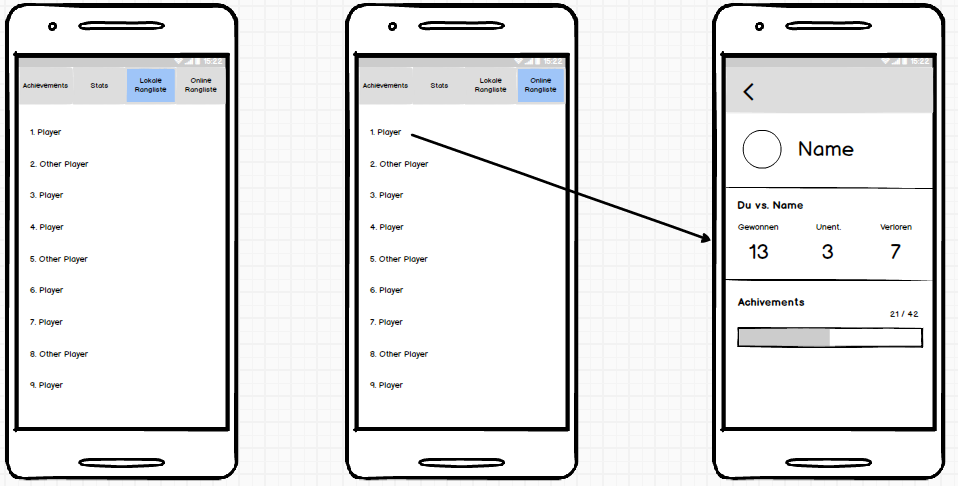
\includegraphics[scale=0.58]{img/mockup_stats_1.png}
	\caption{Statistics Activity}
	\label{stats1}
\end{center}
Außerdem haben wir Mockups zu den Statistiken erstellt. Hier kann der Benutzer
seine bisherigen Erfolge einsehen. Diese Activity ist auf den Abbildungen
~\ref{stats1} und ~\ref{stats2} zu sehen
\end{figure}

\begin{figure}[!ht]
\begin{center}
\centering
	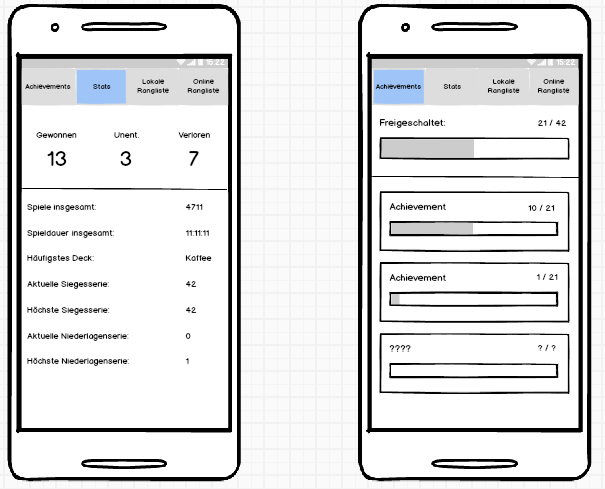
\includegraphics[scale=0.75]{img/mockup_stats_2.png}
	\caption{Statistics Activity}
	\label{stats2}
\end{center}
\end{figure}

\clearpage

\section{Implementierung}
\subsection{Ausgewählte Implementierungsdetails}
\subsubsection{Galerie}

\begin{figure}[!ht]
  \centering
  \begin{minipage}{0.45\textwidth}
    \centering
    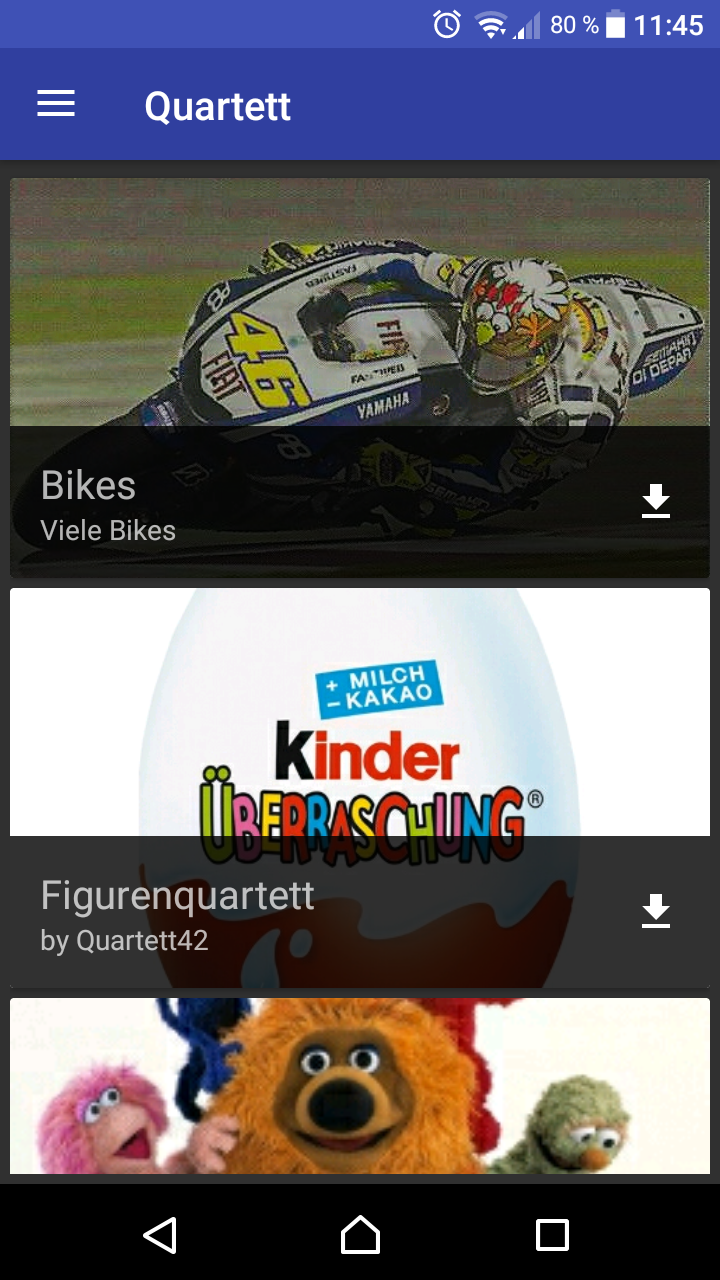
\includegraphics[width=4cm]{img/gallery_decks.png}
    \caption{Deckansicht}
  \end{minipage}
  \hfill
  \begin{minipage}{0.45\textwidth}
    \centering
    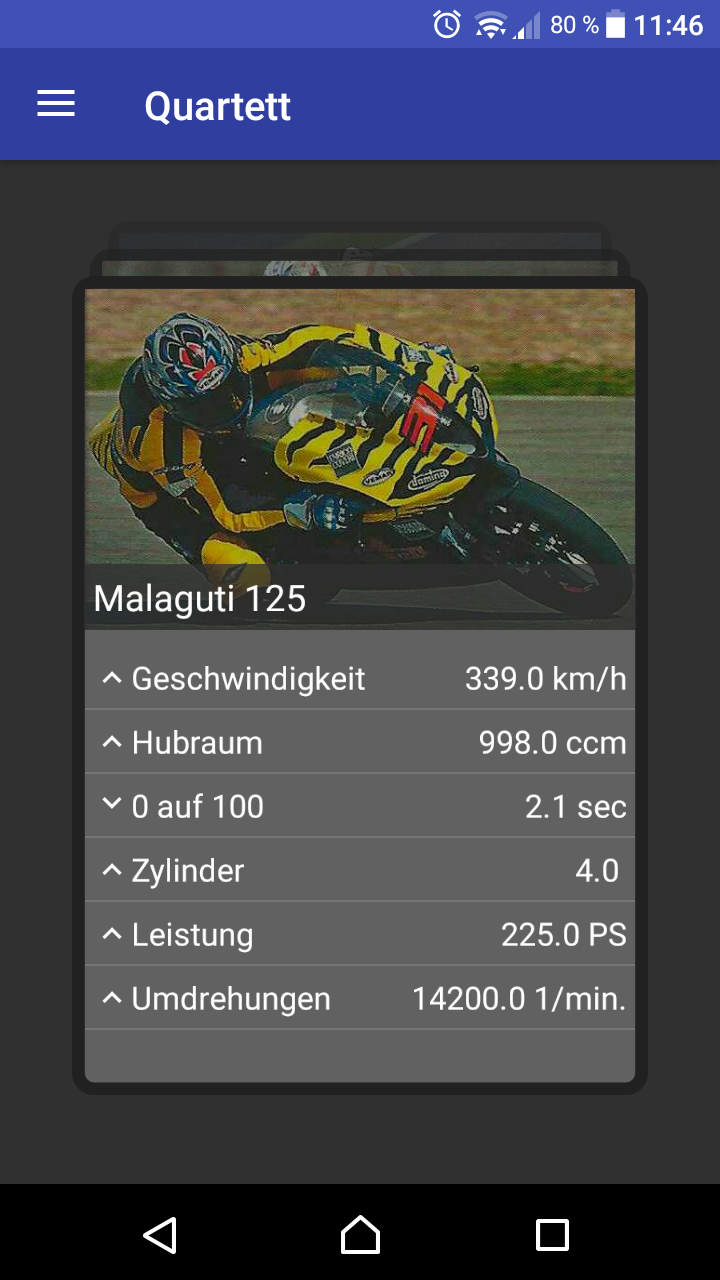
\includegraphics[width=4cm]{img/gallery_cards.png}
    \caption{Kartenansicht}
  \end{minipage}
\end{figure}

\noindent
In der Galerie werden alle Kartendecks aufgelistet, die auf dem Smartphone
vorhanden sind oder vom Server heruntergeladen werden können. Heruntergeladenen
Decks könne durch Antippen geöffnet werden. In der geöffneten Ansicht kann der
Benutzer durch vertikale Wischgesten durch die einzelnen Karten des virtuellen
Kartenstapels blättern. Tippt der Benutzer ein Deck an, welches nicht
heruntergeladen ist, wird ein Dialog geöffnet in welchem das Herunterladen des
Decks bestätigt oder abgelehnt werden kann. Das Deck wird nicht direkt geladen,
da sich der Benutzer eventuell in einer Netzwerkumgebung befindet, in welcher
durch Downloads Kosten entstehen können. Durch den Bestätigungsdialog wird dem
Benutzer somit eine Möglichkeit gegeben den Download zu einem späteren Zeitpunkt
mit günstigeren Netzwerkbedingungen zu starten. Wird der Dialog bestätigt startet
der Download des Decks. Im Listenelement des Decks wird ein Ladebalken angezeigt
und im Notification Drawer wird eine Notification erstellt die ebenfalls den
Fortschritt des Downloads anzeigt. Nach erfolgreichem Download wird die
Notification geschlossen und der Ladebalken verschwindet wieder. Das Deck ist
dann persistent auf dem Gerät gespeichert und kann nun auch ohne
Internetverbinung angezeigt werden. Zudem können nun auch die Karten des Decks,
wie oben beschreiben angezeigt werden. Auch kann das Deck nun im Einzelspieler
Modus verwendet werden.

\begin{figure}[!ht]
  \centering
  \begin{minipage}{0.45\textwidth}
    \centering
    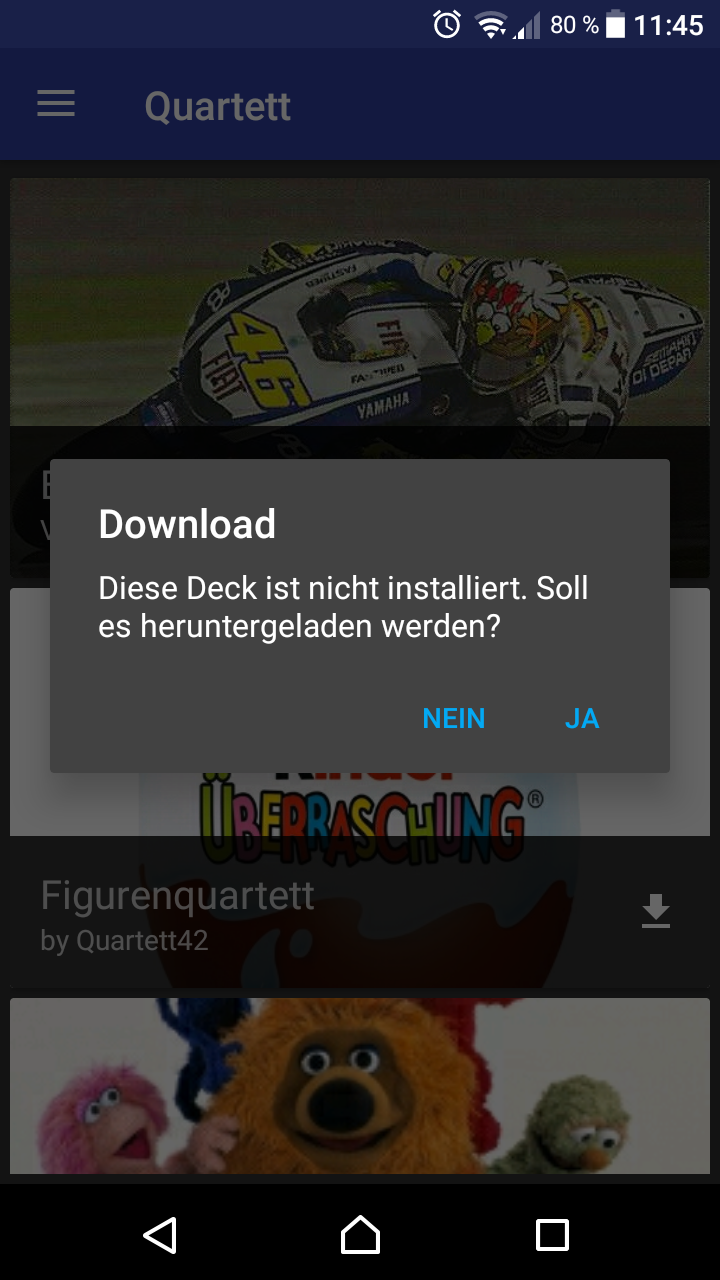
\includegraphics[width=4cm]{img/gallery_dialog.png}
    \caption{Download-Dialog}
  \end{minipage}
  \hfill
  \begin{minipage}{0.45\textwidth}
    \centering
    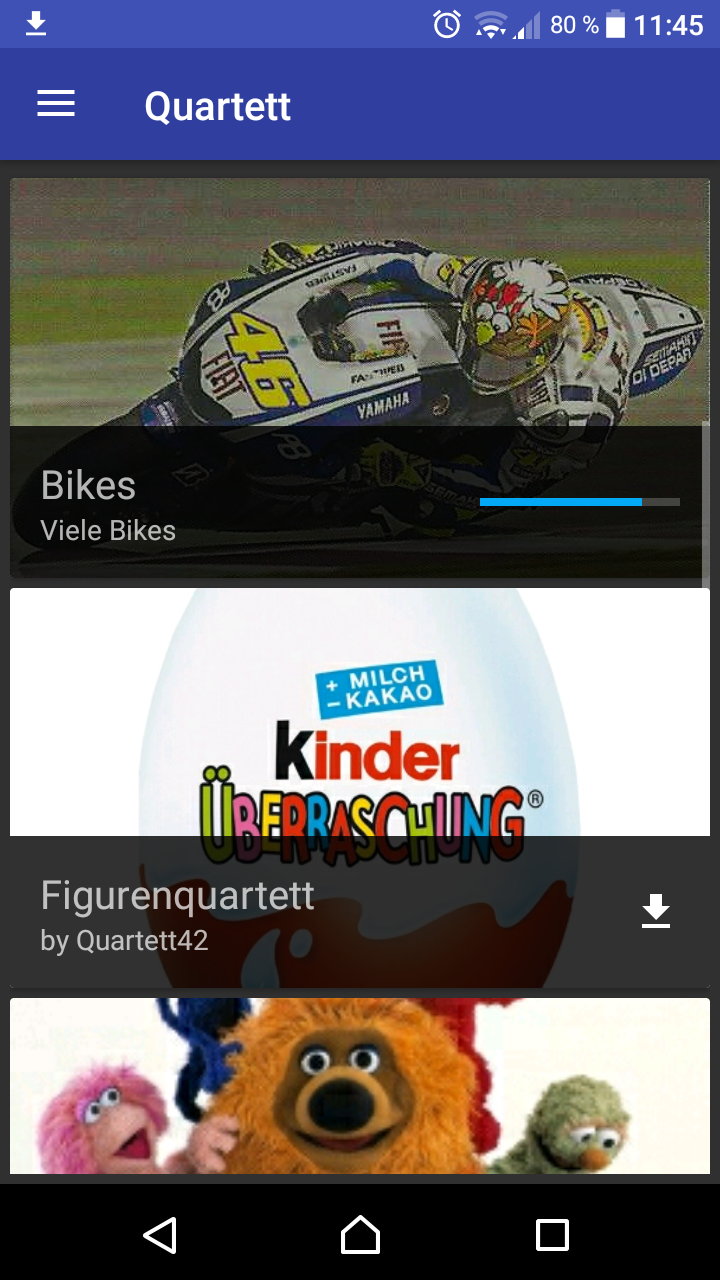
\includegraphics[width=4cm]{img/gallery_download.png}
    \caption{Download-Fortschritt}
  \end{minipage}
\end{figure}

\ \newline
Um die Galerie mit diesen beschriebenen Funktionen zu realisieren, waren einige
besondere Implementierungsmethoden notwendig. Da den meisten Decks und Karten
relativ hochauflösende Bilder zugeordnet sind, entstehen beim Anzeigen der Decks
bzw. Karten Verzögerungen, da große Datenmengen geladen werden müssen. Dabei ist
außerdem zu erwähnen, dass das Laden der Bilder der Decks, die nicht auf dem
Gerät gespeichert sind, über das Netzwerk erfolgt und somit zusätzliche
Verzögerungen entstehen. All diese Verzögerungen sind als starke Ruckler
bemerkbar und beinträchtigen das Nutzererlebnis erheblich. Das Laden der Bilder
wurde daher auf einen zweiten Thread ausgelagert. Somit kann der Benutzer
weitere Interaktion vornehmen während im Hintergrund die Bilder nachgeladen
werden. Auch der Download eines Decks verwendet einen eigenen Thread, um
Verzögerungen im Haupt-Thread der Applikation zu vermeiden. Zusätzlich wurde
hier auch das Service Modell der Android Platform verwendet. So kann garantiert
werden, dass der Download abgeschlossen wird, auch wenn die Galerie verlassen
oder die App während des Downloads geschlossen wird. Um die heruntergeladenen
Daten in der Datenbank zu speichern war ebenfalls eine besonderer Strategie
nötig. Die Daten können nicht sofort gespeichert werden, da sonst bei Fehlern
inkonsistente Zustände in der Datenbank auftreten. Daher werden geladene Daten
zunächst im RAM gehalten bis der Download vollständig abgeschlossen ist und dann
in einer einzigen Transaktion in die Datenbank geschrieben. Somit wird immer ein
konsistenter Zustand der Datenbank erreicht und Fehler können einfacher
abgefangen werden.

\subsubsection{Einzelspieler}

\begin{figure}[!ht]
  \centering
  \begin{minipage}{0.45\textwidth}
    \centering
    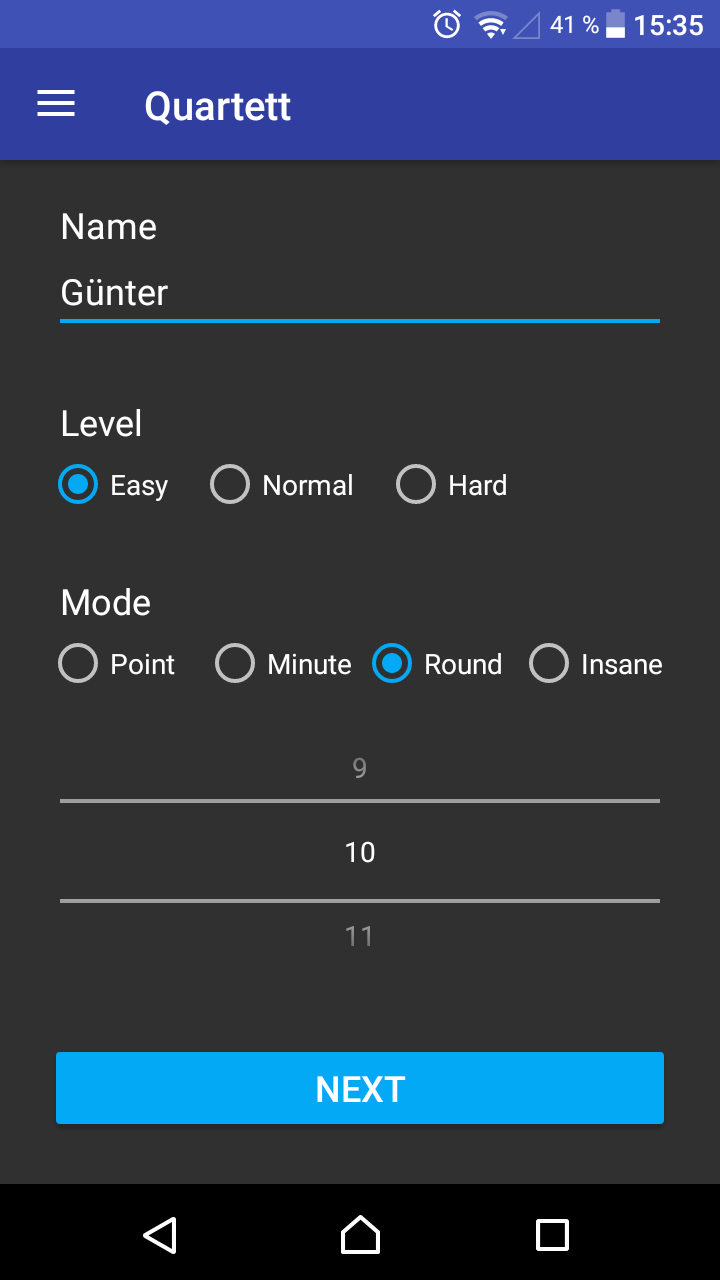
\includegraphics[width=4cm]{img/game_settings.png}
    \caption{Spieleinstellungen}
  \end{minipage}
  \hfill
  \begin{minipage}{0.45\textwidth}
    \centering
    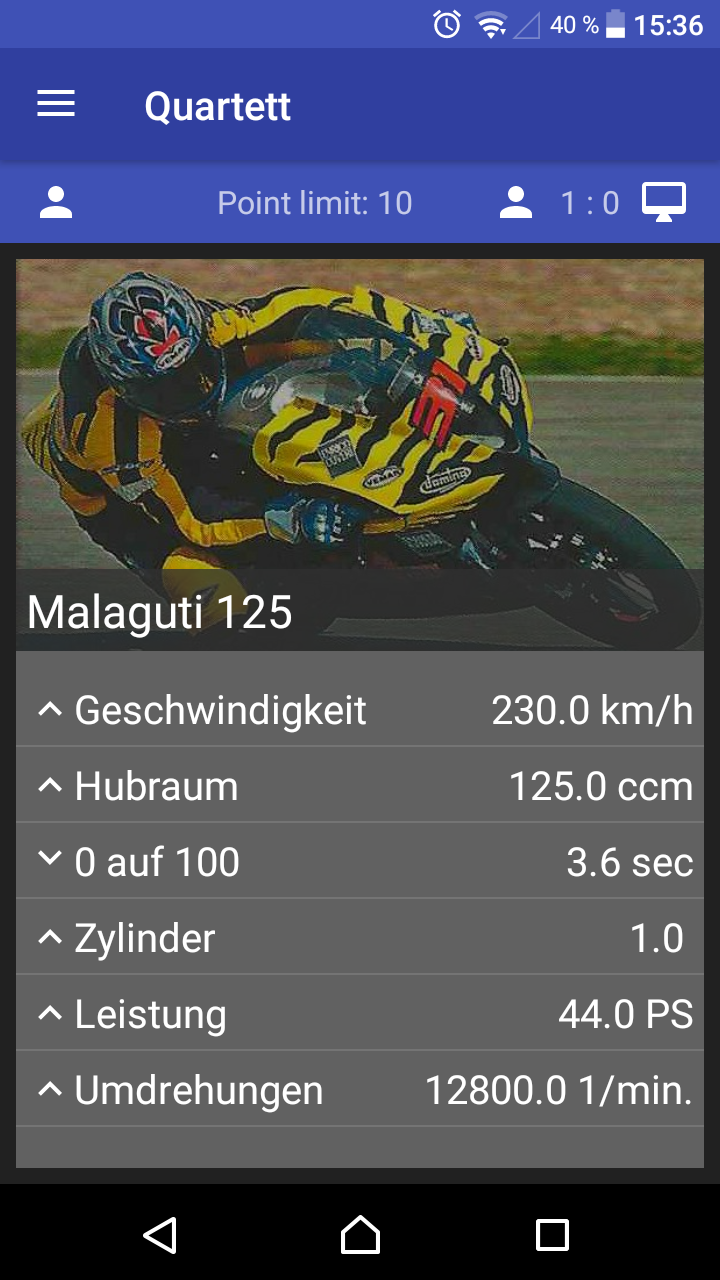
\includegraphics[width=4cm]{img/game_attributes.png}
    \caption{Attributauswahl}
  \end{minipage}
\end{figure}

\noindent
Im Einzelspielermodus der Quartett App werden vor jedem Spiel zunächst einige
Spieleinstellungen abgefragt. Der Name des Spielers wird für den Eintrag in die
lokale Rangliste verwendet. Außerdem kann der Schwierigkeitsgrad, also die
Stärke der KI, und der Spielmodus eingestellt werden. Um die Einstellungen nicht
bei jedem Spielstart erneut setzen zu müssen können Standardwerte für jeden
Parameter in den allgemeinen Spieleinstellungen hinterlegt werden. Nachdem alle
Einstellungen getroffen wurden wird der Spieler aufgefordert ein Deck
auszuwählen, mit welchem das Spiel gestartet werden soll. Dabei stehen nur Decks
zur Auswahl die bereits heruntergeladen worden sind. Nach der Auswahl eines
Decks startet das eigentliche Spiel. Dem Spieler wird eine Karte angezeigt, von
welcher ein Attribut ausgewählt werden kann. Dieses Attribut wird mit dem
Attribut verglichen, das die KI ausgewählt hat. Je nach Wert und Art des
Attributs gewinnt oder verliert der Spieler die Karte. Das Ergebnis des
Vergleichs wird in einer eigenen Ansicht präsentiert. Dort werden die beiden
Karten gegenüber gestellt und Gewinner (grün) und Verlierer (rot) entsprechend
eingefärbt. Hat der Spieler gewonnen so darf er erneut das Attribut bestimmen,
sonst wird der nächste Zug durch die KI ausgeführt. Ist schließlich die
Abbruchbedingung des Spiels erreicht (Zeit, Punkte, Runden) wird das Spiel
beendet und eine Punktezahl berechnet. War der Spieler besonders gut wird
außerdem automatisch ein Eintrag in der Rangliste vorgenommen. Danach besteht
die Möglichkeit das Spiel mit den selben Einstellungen erneut zu starten, die
Einstellungen zu ändern, oder in das Hauptmenü zurückzukehren.

\begin{figure}[!ht]
  \centering
  \begin{minipage}{0.45\textwidth}
    \centering
    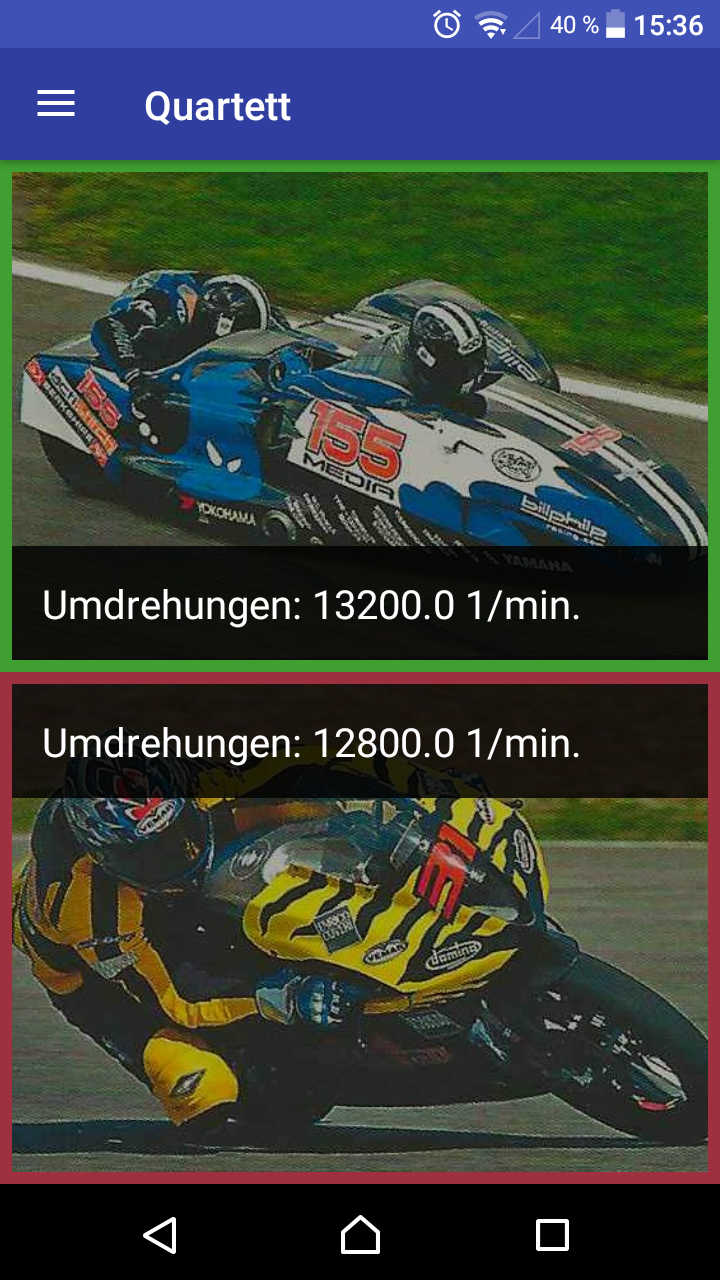
\includegraphics[width=4cm]{img/game_compare.png}
    \caption{Vergleichsansicht}
  \end{minipage}
  \hfill
  \begin{minipage}{0.45\textwidth}
    \centering
    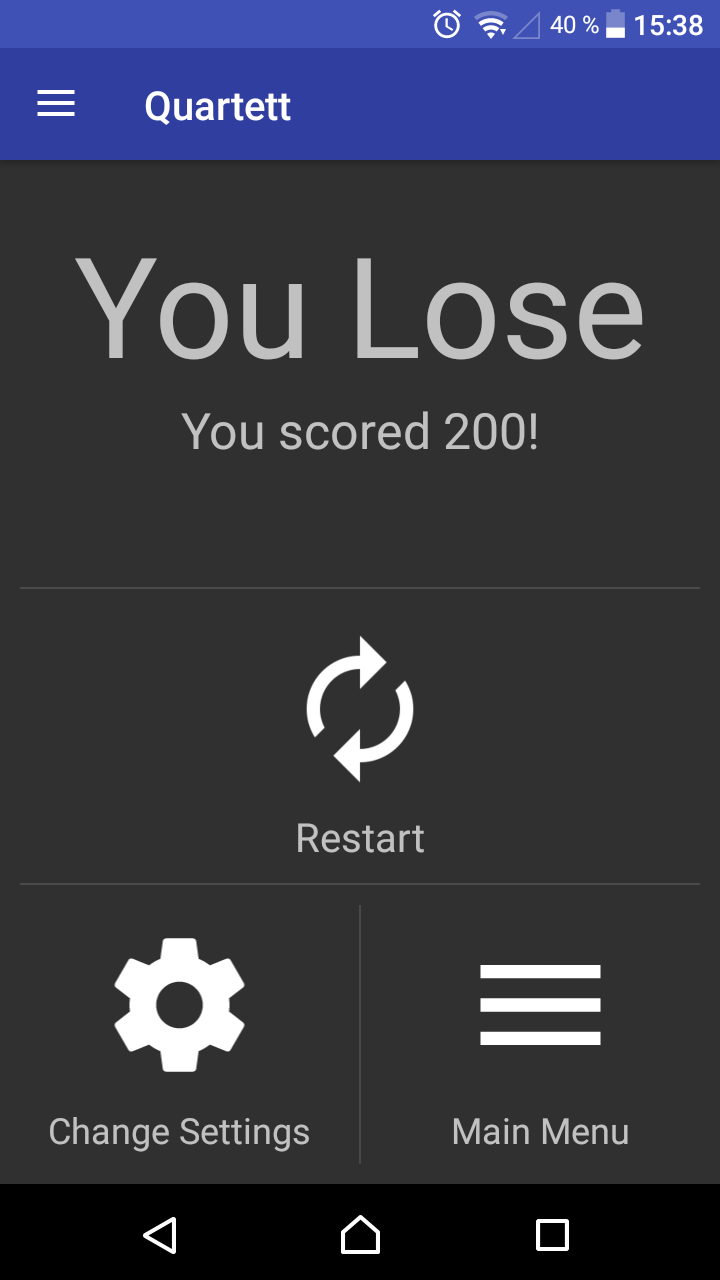
\includegraphics[width=4cm]{img/game_end.png}
    \caption{Spielende}
  \end{minipage}
\end{figure}

\noindent
Bei der Implementierung des Einzelspielers war besonders die KI eine
Herausforderung. Diese musste sich möglichst wie ein Spieler verhalten und kein
unfaires Spielerlebnis bieten, also nicht zu viel Wissen über den Spielstatus
erhalten. Die hier verwendete Implementierung erzeugt zunächst für jedes
Attribut eine nach eben diesem Attribut sortierte Liste der Karten. Danach wird
die Position der Karte in jeder dieser Listen ermittelt und dem jeweiligen
Attribut zugeordnet. Damit weiß die KI nun welches der Attribute das
\enquote{beste}, also das mit den höchsten Gewinnchancen ist. Je nach
eingestelltem Schwierigkeitsgrad wird die KI dann eher bessere oder eher
schlechtere Attribute auswählen. So wird ein Spieler simuliert, der das
Kartendeck, je nach Schwierigkeitsgrad, mehr oder weniger gut kennt, somit
abschätzen kann wie \enquote{gut} ein Attribut ist und auf Basis dieser
Schätzung seine Entscheidungen trifft. Außerdem erhält die KI mit dieser
Implementierung auch nicht mehr Informationen als ein menschlicher Spieler.
Unfaires Verhalten wird somit verhindert.

\subsubsection{Multiplayer}
Der Multiplayer bietet den Spielern die Möglichkeit über eine Internetverbindung
gegeneinander zu spielen. Entscheidet sich der Nutzer zu einem Multiplayer Spiel
gelangt dieser zu erst auf eine Activity die ihm eine Liste aller Spiele anzeigt
die er gerade spielt und auch die Möglichkeit gibt ein neues Spiel zu starten.
Wählt der Nutzer ein neues Spiel kann er sich entscheiden ob er automatisch
einem anderen Spieler zugeteilt werden möchte oder gezielt mit einer bestimmten
Person spielen möchte.

\ \newline
Im Mulitplayer-Modus wird im Gegensatz zum herkömmlichen Quartett immer
abwechselnd gespielt egal wer die vorherige Runde gewonnen hat. Dies ist eine
Designentscheidung die aus Usability Gründen getroffen wurde. Andernfalls könnte
es vorkommen ein Spieler macht einen Zug, schließt die App um später weiter zu
spielen aber in der Zwischenzeit gewinnt sein Gegner alle folgenden runden und
beendet das Spiel ohne, dass der erste Spieler etwas mitbekommt.

\ \newline
Die technische Umsetzung wurde durch die bereits im Kapitel Libaries und
Frameworks erwähnten Google Play Services extrem erleichtert. Durch die
Verwendung dieser Services mussten wir uns nur noch um den client-seitigen Teil
der Anwendung kümmern. Hier war der anspruchsvollste Teil jedes mögliche
Szenario abzudecken. Also entsprechend zu reagieren wenn einer der Spieler einen
Zug gemacht hat und der andere zum Beispiel gerade noch das Ergebnis des
vorherigen Zuges angeschaut hat oder gar nicht mehr innerhalb der App war. Da
Quartett ein rundenbasiertes Spiel ist war die Synchronisation eher trivial.
\subsection{Architektur}
\subsubsection{Datenmodell}

\begin{figure}[h]
  \centering
  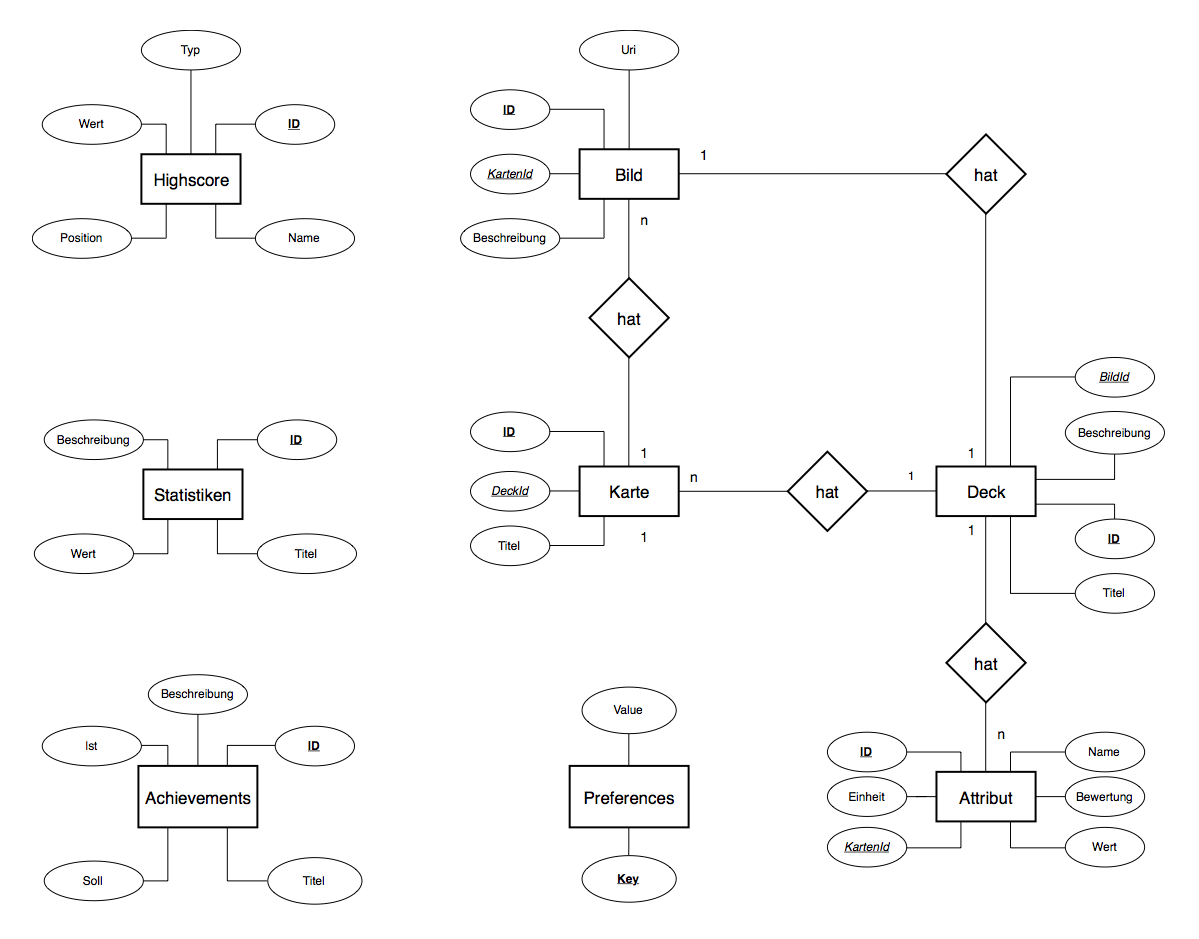
\includegraphics[width=\textwidth]{img/map_er.png}
  \caption{ER Diagramm des Datenmodells}
\end{figure}

\noindent
Im obigen ER Diagramm ist die Struktur unseres Datenmodells dargestellt. Zur
Realisierung wurde die in Android integrierte SQL Datenbank SQLite in
Kombination mit Sugar ORM verwendet. So konnten die einzelnen Entitäten direkt
über Klassen angesprochen werden und es mussten keine SQL Statements verwendet
werden. Allerdings beherrscht Sugar ORM in der verwendeten Version keine Listen
und Beziehungen zwischen den einzelnen Entitäten können mit Sugar ORM ebenfalls
nur schwierig oder gar nicht dargestellt werden. Die Daten der gespeicherten
Bilder wurden nicht in die SQL Datenbank geladen sondern direkt im internen
Speicher des Geräts abgelegt. Auch die \enquote{Preferences} werden nicht mit
SQL gespeichert sondern in den SharedPreferences des Android Systems abgelegt.
SharedPreferences ist eine einfach Key-Value Datenbank die sich kleine
Datenmengen eignet.

\subsubsection{Klassenstruktur}

\begin{figure}[!ht]
  \centering
  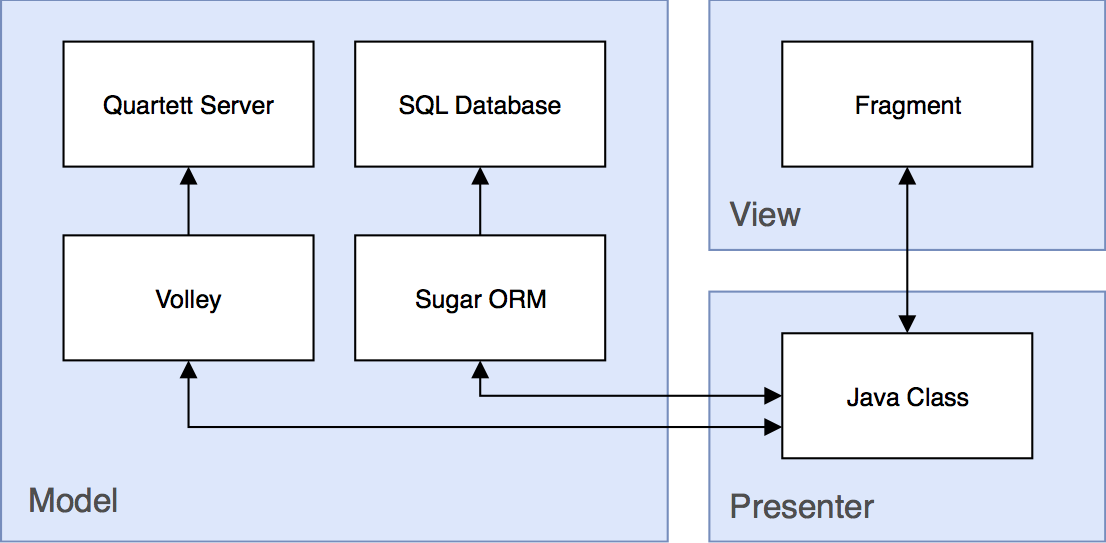
\includegraphics[width=\textwidth]{img/class_structure.png}
  \caption{Schematische Klassenstrukur der App mit MVP-Pattern}
\end{figure}

\noindent
Um die Applikation zu strukturieren wurde hier das Model-View-Presenter Pattern
angewendet. Mit diesem Pattern wird jede Activity in Model-, View- und
Presenter- Komponenten zerlegt. Die Model Komponenten beinhalten die
Zugriffsschicht auf die Datenbank mit allen zugehörigen Klassen. In der hier
vorgestellten App wird das Model durch Sugar ORM bzw. durch dessen
Entitätsklassen dargestellt. Außerdem wird die Serveranbindung, welche durch das
Volley Framework realisiert wird, ebenfalls zum Model gezählt. Es existiert
nur ein gemeinsames Model für alle Activities. Auf das Model kann nur vom
Presenter aus zugegriffen werden. Dieser verwaltet die
eigentlich Logik einer Activity. Dabei ist der Presenter selbst eine einfache
Java Klasse ohne direktes Wissen über das Android System oder die Datenbank.
Events der View werden an den Presenter weitergeleitet und dort bearbeitet. Der
Presenter kann zur Bearbeitung von Events sowohl auf das Model als auch auf die
View Komponenten zugreifen. Diese Komponenten beinhaltet die Anzeigeschicht und
verwaltet die einzelnen GUI-Elemente. In unserer App wird die View von einer
Fragment Klasse implementiert. Direkt kommuniziert die View nur mit dem
Presenter und greift nicht auf das Model zu. In der Praxis gibt es dabei
allerdings einige Ausnahmen.

\ \newline
Um z.B. das Anzeigen von Listen in Android effizient zu realisieren werden
sogenannte Adapter verwendet. Diese greifen meist direkt auf die Datenbank zu
und stellen die erhaltenen Daten direkt in einer ListView da. Damit können diese
Klassen nicht eindeutig den Model oder View Komponenten zugeordnet werden. Daher
implementieren diese meist sowohl die Eigenschaften des Models als auch der
View.

\ \newline
Durch die klare und immer gleichförmige Strukturierung in Model, View und
Presenter, wird das Erstellen von neuen Activities vereinfacht, da somit ein
klarer Arbeitsablauf gegeben ist. Auch das lesen und editieren von fremden Code
wird erleichtert, da von vornherein anhand der Benennung der einzelnen Klassen
klar ist welche Aufgaben diese Komponenten übernehmen.

\section{Anforderungsabgleich}

Im Folgenden werden die gegebenen Anforderungen mit der tatsächlichen
Implementierung verglichen. Es wird festgestellt ob eine Anforderung ganz,
teilweise oder gar nicht erfüllt wurde.

\subsection{Funktionale Anforderungen}

\textbf{FA1 Hauptmenü - erfüllt} \newline
Das Hauptmenü wurde wie in der Anforderung beschrieben implementiert.

\ \newline
\textbf{FA2 Spielmodi - erfüllt} \newline
Alle Spielmodi wurden wie gefordert implementiert und können vor jedem Spiel
ausgewählt werden.

\ \newline
\textbf{FA3 Computergegner - erfüllt} \newline
Für den Einzelspielermodus wurde ein Computergegner implementiert, der ein
faires Spielerlebnis bietet. Diese \enquote{KI} kann je nach Schwierigkeitsgrad
unterschiedlich gut abschätzen welches Attribut einer Karte die höchsten
Gewinnchancen hat und imitiert so das Verhalten eines menschlichen Spielers.

\ \newline
\textbf{FA4 Schwierigkeitsgrad - erfüllt} \newline
Die geforderten Schwierigkeitsgrade wurden implementiert und können vor dem
Beginn eines neuen Spiels ausgewählt werden. Die Wahl des Schwierigkeitsgrads
beeinflusst das Verhalten der KI.

\ \newline
\textbf{FA5 Spiel fortsetzen - erfüllt} \newline
Nach jedem Spielzug wird der komplette Zustand des Spiels in die interne
Datenbank geschrieben und damit persistent gespeichert.

\ \newline
\textbf{FA6 Galerie - erfüllt} \newline
Die Galerie wurde wie in \enquote{Implementierungsdetails} beschreiben
implementiert.

\ \newline
\textbf{FA7 Deck Download - erfüllt} \newline
Der Deckdownload wurde wie in \enquote{Implementierungsdetails} beschreiben in
die Galerie integriert.

\ \newline
\textbf{FA8 Statistiken - erfüllt} \newline
Die Statistiken wurden implementiert und werden graphisch aufbereitet in einer
speziellen Ansicht dargestellt.

\ \newline
\textbf{FA9 Rangliste - erfüllt} \newline
Die beschriebene Rangliste wurde implementiert. Der Spieler wird mit dem Namen
der zu Beginn eines Spiels eingegeben wurde, automatisch mit seiner erreichten
Punktezahl in die Rangliste aufgenommen

\ \newline
\textbf{FA10 Achievements - teilweise erfüllt} \newline
Es wurde eine Oberfläche zur Anzeige der Achievements implementiert. Ein
fertiges Achievementsystem ist allerdings nicht in der App vorhanden.

\ \newline
\textbf{FA11 Quartetteditor - nicht erfüllt} \newline
Der Quartetteditor wurde zugunsten des Multiplayers nicht realisiert.

\ \newline
\textbf{FA12 Levelsystem - nicht erfüllt} \newline
Das Levelsystem wurde zugunsten des Multiplayers nicht realisiert

\ \newline
\textbf{FA13 Multiplayer - erfüllt} \newline
Der Multiplayer wurde mit Hilfe der Google Play Services implementiert und
erlaubt es zwei Benutzer der App über das Internet gegeneinander anzutreten.

\subsection{Nicht Funktionale Anforderungen}

\textbf{NFA1 Robustheit - teilweise} \newline
Der Multiplayer weist aufgrund der Komplexität und fehlender Entwicklungszeit
noch einige Stabilitätsprobleme auf. Ansonsten konnten während der Entwicklung
keine Fehler festgestellt werden, welche die Robustheit der App beinträchtigen.

\ \newline
\textbf{NFA2 Erweiterbarkeit - erfüllt} \newline
Durch die Verwendung des Model-View-Presenter Patterns ist eine einfache
Erweiterbarkeit gegeben.

\ \newline
\textbf{NFA3 Responsiveness - erfüllt} \newline
Durch den permanenten Einsatz von asynchronen Programmiertechniken wurde
sichergestellt, dass die Applikation immer entsprechend schnell reagiert.

\ \newline
\textbf{NFA4 Usability - erfüllt} \newline
Um die Usability sicher zu stellen wurden die Google User Interface Guidelines
als Referenz für die Gestaltung der Oberflächen verwendet.

\section{Zusammenfassung und Ausblick}

In dieser Dokumentation wurde die Planung der Entwicklung einer Android Quartett
App und die tatsächlich Implementierung dieser vorgestellt. Da die allermeisten
der funktionale und nicht funktionalen Anforderungen erfüllt wurden, kann das
Projekt als erfolgreich bewertet werden. Darüberhinaus konnten wir zahlreiche
Einblicke in die Entwicklung von Android Applikationen erhalten. Wir sind nun
mit den wichtigsten Konzepten der Plattform vertraut, sodass die Entwicklung
weiterer Apps deutlich einfacher zu bewerkstelligen sein wird. Außerdem konnten
wir zusätzliche Erkenntnisse in der Verwendung von Design Patterns und des
Versionskontrollsystems git sammeln.

\ \newline
Aufgrund der gewonnen Erkenntnisse und des allgemein guten Projektverlaufs werden
wir auch weiter Apps mit Android und unter zu Hilfenahme der hier verwendeten
Werkzeuge und Strategien entwickeln.

\end{document}
